\documentclass[12pt]{article}
\usepackage{amsmath}
\usepackage[dvipdfm]{graphicx}
\usepackage{bmpsize}
\usepackage{color}
\usepackage{hyperref}
\usepackage{float}
\usepackage{verbatim}
\usepackage{alltt}
\author{andruiman, \href{maito: andruiman@gmail.com}{andruiman@gmail.com}\footnote{To support this work please use our asset in AE: 5841059555983208287}}
\title{PoS forging algorithms: formal approach and multibranch forging}
\newcommand{\begver}{\begin{alltt}\begin{footnotesize}}
\newcommand{\enver}{\end{footnotesize}\end{alltt}}

\begin{document}

\maketitle
\begin{abstract}
In this paper we present the concept of provable code usage for formally described and reliable crypto-currencies systems development. 
As a demonstration of this approach, a model of a multibranch forging algorithm in a Proof-of-Stake network is presented. 
The results of simulation show the potential power of multibranch forging as well as a potential tendency towards the 
Proof-of-Work networks which should be avoided. The latter opens new areas of research. Our concept of the multibranch forging can be interpreted 
as a formally stated reference implementation for the broadly discussed Transparent Forging model. Examples of functional code are also presented to 
demonstrate our approach and its properties.
\end{abstract}

\noindent
{\bf Keywords:} PoS crypto-currencies, forging, blocktree, simulation

\section{Pre-introduction}
We continue the series of papers on various aspects of Proof-of-Stake forging algorithms. We act as the Consensus Research 
Group \url{http://consensusresearch.org} and publish our updates both on the website and the Nxt forum \url{https://nxtforum.org/consensus-research/}.
We plan to concentrate on one result in each paper and update our status with at least one new paper or software upload every two weeks describing 
what we will have achieved. For the papers that need corrections or important changes we will update in the usual way,
issuing the next versions. 

\section{Introduction or Time for definitions}
The world of crypto-currencies (CC) is one of the most innovative and progressive field both for research 
and software development in financial sphere based on liberty and independence. However new areas sometimes suffer from unproved methods and speculations.  
To bring a new branch of discussions based on verifiable statements we offer the community to summarize what we already know and give the more or less formal 
definitions to broad used terms. We realize that the definitions always restrict something but from the opposite side they bring a common knowledge and let people 
to use the same terms meaning the same things. The most powerful way to give definitions is using mathematical models of what we investigate and introduce the 
terms as strict math formulations and the statements as theorems. The approach of building on formal mathematical definitions allows
for a much deeper understanding and give a common ground for discussions. Unless the definitions of the basic terms are made clear and explicit,
disagreeements in discussions are often based on misunderstandings.

It is important to note is that CC is already an industry. The community surrounding CC awaits not just a theory but an executable software which brings 
the required properties. We are lucky that actually we have already developed tools to do both at the same time. One
of the approach is the use of proof assistant systems which let developers to proof the statements and get the executable code as a final result. However these 
systems sometimes restrict the development process. In particular programmers are often forced to use functional representations of code and inductively 
defined datatypes with strictly decreasing recursion (statically ensuring termination). Such restrictions are not broadly accepted by programmers. 
Our goal here is to create reference implementations of some algorithms which could be interesting for research and translating them to more acceptable 
forms of code. Another way is to use proof assistants to develop the core of a system or its most critical parts. 
So summarizing, our principle of development is as follows:
$$
{\rm Principles\ of\ the\ system}\to{\rm Definitions\ \&\ strict\ specification}\to
$$
$$
\to{\rm Reference\ code}\to{\rm Proof\ of\ specification}\to{\rm Executable\ version}.
$$  

This paper is to show the main result concerning the multibranch forging as well as to demonstrate our way of development. The proof assistant system we use is 
Coq \url{https://coq.inria.fr/} and the reference language is Haskell \url{https://www.haskell.org/haskellwiki/Haskell} so we use both languages notations 
for convenience. We sassume that a reader is familiar with functional notations however the results of the paper can be understood without this knowledge. 
We also assume that a reader is familiar with basics of crypto-currencies technology so we describe only the concepts important for this paper.

\section{PoX forging and blocktrees}
Most existing CCs use one of the following principles to build a blockchain \-- Proof-of-Work or Proof-of-X, where X is not Work, 
and there are also hybrid 
systems using both of them. The main difference between these principles is that in PoW systems the right to generate block arises 
when a certain calculations (work) are made and in PoX systems the right arises based on logical and/or directly measurable parameters of the generating account. 

One of the most popular principles is the PoS 
(Proof-of-Stake) system where the right to generate a block arises from a certain amount of stake (portion of coins) which 
an account accumulates and some predefined mechanism for generating and accepting blocks. The question we begin to investigate here is a 
general possibility and modeling results of PoS forging in a special environment. Almost all the CC systems use the so called blockchain as a 
main dynamic structure to store the network specific data. A blockchain is a sequence of blocks used with the following purposes: (1) each block contains the 
accumulated network specific information such as transactions and other valuable data which have to be shared between the peers 
(2) blocks are connected in the cause and effect principle. So the later block cannot exist without
the previous: $\forall a_1,a_2\in A, (a_1\Rightarrow a_2) \to (a_1\in B_1) \to (a_2\in B_2) \to B_1 \prec B_2$. We denote with $A$ a set of possible actions or 
events stored in the block and denote with $a_1\Rightarrow a_2$ the fact that an event $a_2$ is dependent (or cannot be occur without) an event $a_1$. 
The sequencing of the
blocks we denote as $B_1 \prec B_2$ meaning strict following of the $B_2$ after $B_1$ in the blockchain. The latter proposition we can write with a weak form of
$B_1 \preceq B_2$ but to avoid postponing processing events (due to the asynchronous way actions are processed) it is better to use the strict form.
It should be noted
that actions are not ordered based on the time of creation, the only thing we need is the causing conditions and the fact that every action 
will be put in a blockchain within a certain time interval. 

The procedure of blocks generating in the PoS systems is called forging. The difference between PoW and PoS systems arises when we think
of what block to build. Actually each account running a node in the network is generally speaking free to choose what to do \-- the only thing we can claim from it
is to follow a certain protocol to belong to a certain CC network. In the PoW systems there exist the most powerful branch and nodes choose to 
build a block on the top of the last block in this chain because they cannot build on several branches with the same computational power. That is a way 
to create a network consensus \--
roughly speaking, an account (or node) who decided to build a block in other place should be more powerful or lucky 
than all the nodes who decided to build a "right-placed" block and therefore
the winning strategy is most probable to act as others. 
The latter could be called "consensus in acting" when doing the same things will benefit all parties in getting 
the result. The weaker form of consensus can be called "consensus in vision" when we get the same result (e.g. accounts' balances) 
doing theoretically different things (e.g. forging to different branches, but keeping the whole tree). The weakest form of consensus could be observed when 
peers have {\it different} internal data ("the intermediate result") which is nevertheless equally (or equivalently) interpreted.
 
Note that in the PoS systems we cannot force the nodes to do the same things at all because they don't lose anything (like computing power in PoW) doing 
different things at the same moment, for example forging to different branches of the blockchain. And the question is \-- could we in principle achieve a rational
consensus at its weak form in the pure PoS system? At the moment we are a few steps before we can give a strict definition to the consensus itself and its form. 
And thus we allow ourselves to be inspired from the simulation of multibranch forging in PoS systems as a way to demonstrate a process of the natural 
blockchain forking. To do this we introduce a blocktree \-- a tree-like structure of blocks without 
forcing it to be a list (a chain) as its best. A blocktree is data which each node can locally store and exchange with others like with the blockchain. 
The only thing we need from this tree is to have a possibility to create the present vision of reality or just choose the one. 
The consensus for such a network means that nodes benefit from choosing the same vision. The cause
and effect principle surely should be held for a tree as well as for a chain. 

We continue our general constructions in future works and start describing the concrete system from this point.

\section{Blocktree forging and Transparency}
The main idea of Transparent Forging is that accounts can choose between generating a block or skipping 
their turn to all-the-network benefits. 
It is possible because in some circumstances the future forgers are more or less known and possible future is predictable. So looking to the future block generation
process an account can choose its strategy based on its belief. However not going deeper into implementation of exactly this idea and living in the 
transparent environment let's switch the rule to "If you can generate - do it and tell others, but you may keep several versions of a future". It is easy to see
that is almost the same principle \-- if an account can generate a block at the given time it anyway generates it but the outgoing block 
can be interpreted as only one of possible outcome from the previous. Other accounts still have a right to forge to the previous block and generate a 
new block later (but maybe "better"), and they also will tell the 
network about their efforts. So we change the rule "predict and decide" to the rule "act and choose later". This is possible because predicting here means the
same as acting for all forging accounts, so if all accounts act \-- they all predict. 

We realize a little difference between the original "generate/skip" and multibranch strategies but 
we think it is not principal. We do not discuss the security here \-- we think the security lies beyond the forging algorithms (we'll discuss it in separate 
paper). So our blocktree forging is a kind of Transparent Forging implementation with shifted aspects. We offer not to decide which future is better for the 
network (or account) now \-- we offer to keep them all and choose later. This approach gives the peers an independence on prediction 
quality and allows not to suffer from the wrong predictions. So we give the formal description of our model below and it can be also 
interpreted as a formal description of TF in our vision.

\section{Blocktree structures and forging}
We use the Nxt forging algorithm as a reference one and change only the block storing structure. To be compatible with the list (chain) we define our blocktree as a 
following \texttt{LTree} datatype:
\begver
Inductive LTree (X: Type) : Type :=
| tgen : X -> LTree X
| tcons : X -> LTree X -> LTree X
| tfork : LBranch X -> LTree X -> LTree X  with 
  LBranch (X: Type) : Type := 
  | tbranch : LTree X -> LBranch X.
\enver
So we have three ways to construct the \texttt{LTree} data: (1) to create a vertex using \texttt{tgen} (2) to add a vertex to the end like in lists using
\texttt{tcons} constructor (3) to fork the last vertex with another \texttt{LTree} using the \texttt{tfork} constructor. We use the the simple datatype
\texttt{LBranch}$\sim$\texttt{LTree} to distinguish between the first and the second arguments in the \texttt{tfork} call in our \texttt{LTree}, so the first is a branch and the 
second is a truck. To simplify the notes we add the following notations to the constructors:
\begver
Notation "t # a" := (tcons a t) 
                     (left associativity, at level 1).
Notation "tl @ tb" := (tfork (tbranch tb) tl) 
                     (left associativity, at level 1).
Notation "< x >" := (tgen x).
\enver 
The polymorphism is added using the abstract type \texttt{X} which in the case of blocktree should be set equal to the network specific \texttt{Block}
type, that is
\begver
Definition Blocktree := LTree Block.
\enver 
Our tree cannot be empty, that is to avoid empty forks and we suggest this doesn't restrict the generality. The main idea to hold such a tree representation
is to have simple possibility to rebalance it to a list form when we have the only main truck with some forks hanging on it. However it is isomorphic to a general 
rose tree:
\begver
Inductive RTree (X:Type) : Type :=
| branch : X -> list (RTree X) -> RTree X.
\enver 
with a predefined \texttt{list} polymorphic datatype:
\begver
Inductive list (A : Type) : Type :=
    nil : list A | cons : A -> list A -> list A.
\enver
So returning to our \texttt{LTree} type we give some examples of notations:
\begver
<0> # 1 # 2 # 3 (*a list of numbers*)
<0> # 1 @ (<11> # 12) # 2 # 3 (*the same with a fork at 1*)
<0> # 1 @ (<11> # 12) @ (<111> # 112) # 2 # 3 (*the same with the second 
                                                fork at 1*)
\enver

We give below some examples of functions we use in our model referring a reader to the repository with source code for full text.
The example of a non-recursive function which cuts a tree tail if any:
\begver
Definition cut_tail {X} (t:LTree X) :=
match t with
| tgen _ => t
| t' # a => t'
| _ @ _ => t
end. 
\enver
That is a very simple function with matching of a tree to possible inductive constructors. It returns the tree without the last vertex if it exists. 

The example of a recursive \texttt{map} which maps some external function \texttt{f} to a whole tree:
\begver
Fixpoint ltree_map {X Y} (f: X -> Y) (t: LTree X) :=
match t with
| tgen a => tgen (f a)
| l # a => (ltree_map f l) # (f a)
| l' @ l'' => (ltree_map f l') @ (ltree_map f l'')
end.
\enver
That is one of the classical function with transparent recursion which let us to have \texttt{Mappable} class if we like. 

The example of a tree grow function which tries to add a new vertex (\texttt{y}) to the given one (\texttt{x}) in all found places:
\begver
Fixpoint forks {X} (ff: list (LTree X)) t := 
match ff with
| [] => t
| fx :: fs => (forks fs t) @ fx
end.

Fixpoint ltree_grow0 {X} (x y: X) (eqX: X -> X -> bool) (t: LTree X) 
                    (bfork: bool) (lbr: list (LTree X)): LTree X :=
match t with
  | tgen a =>  if (eqX x a) then
                  if (bfork) then forks ((tgen y)::lbr) t
                             else (forks lbr t) # y
               else (forks lbr t)

  | l # a => let l' := ltree_grow0 x y eqX l true [] in
             if (eqX x a) then 
                 if (bfork) then forks ((tgen y)::lbr) (l' # a) 
                            else (forks lbr (l' # a)) # y 
             else (forks lbr (l' # a))
 
  | t' @ t'' => let l'' := ltree_grow0 x y eqX t'' false [] in
                    ltree_grow0 x y eqX t' bfork (l''::lbr)                   
end.

Definition ltree_grow {X} (x:X) y eqX t := ltree_grow0 x y eqX t false [].  
\enver
The more complicated function using the helpers \texttt{forks} which merely adds a \texttt{list} of trees to the end of the given tree and the function 
\texttt{ltree\_grow0} with accumulators \texttt{bfork} and \texttt{lbr}. The external boolean equality \texttt{eqX} for \texttt{X} is also given assuming at least:
\begver
Hypothesis eqX_refl: forall x, eqX x x = true.
Hypothesis eqX_comm: forall x y, eqX x y = eqX y x.
Hypothesis eqX_ext: forall (Y: Type) (x y) (f: X -> Y), 
                                     eqX x y = true -> f x = f y.
\enver 

We also introduce an important function \texttt{rebalance} which rebalances the tree to have the longest (with some measure) chain as a main truck but skip 
here the listing to save the paper volume.

With the above defined \texttt{LTree} structure and functions around we redefine the forging algorithm based on the following principles: (1) each forging account
can freely decide what block to forge to (2) the right to forge arises based on the original Nxt \texttt{baseTarget/Hit} principle (3) accounts distribute
a pair of block (parent-child) immediately after generating (4) the current vision is calculated based on the branch with the largest length (or 
alternatively \-- on cumulative \texttt{baseTarget}) which is calculated using \texttt{rebalance} function. 

As we do not have an infinite computing power we need to restrict the number of blocks to forge to. That is a kind of investigation what principle should be applied 
here. We choose the following \-- keeping a list of open blocks (like in A* algorithm for a graph search) we choose from it a certain number \texttt{tfdepth} 
of blocks with maximum \texttt{baseTarget}, and the list of open blocks is updated when receiving new blocks from peers. So we offer a method to solve the trade-off
between choosing newer blocks and more powerful blocks (which lead to a shorter time to the next block due to a larger \texttt{baseTarget}). 
Each time the account generates to a certain block the latter is removed from the open blocks list. We repeatedly have to note that 
this algorithm should become the subject of a study.

\section{Proofs around and Haskell extraction}
We will dedicate a special paper to the Coq programming languages and ways to proof a code. Here we'd like to present an idea how one can use the
pair Coq-Haskell to produce a proved program. So suppose we define all the functions we need to simulate the forging process. The good thing 
is that we can simulate it directly in the Coq IDE on the fly to realize what happens. However Coq interpreter is not very fast and we need some
standalone program which runs our simulation and can communicate with users, files, network etc. For the latter purpose we use the Haskell code extraction.
So why do we need Coq at all? While coding structures like trees it is important to know that we code what we like and have a tool to verify this. With 
Coq it possible to formally define a specification (properties of datatypes and functions) and prove it or realize why it cannot be proved and therefore
a code requires corrections. Let's look at examples. Suppose we define a tree search function \texttt{search\_ltree} which returns 
the position \-- a path on the tree to the searching vertex or nothing if the vertex is not found. 
We use integer numbering for forks, so the path is a list of elementary movements on a tree (type \texttt{branchpos} and \texttt{list} on it).
\begver
Inductive branchpos : Type := 
| mainbr : branchpos
| forkbr : nat -> branchpos.

Definition LTreePos := list branchpos.

Fixpoint search_ltree0 {X} (x: X) (t: LTree X) (eqX: X -> X -> bool) 
                        (pos: LTreePos) (f: nat): option LTreePos :=
match t with
| tgen y => if (eqX x y) then Some (pos++[mainbr]) else None
| tcons y t' => if (eqX x y) then Some (pos++[mainbr]) 
                        else search_ltree0 x t' eqX (pos++[mainbr]) 0
| tfork (tbranch t'') t' => 
          match search_ltree0 x t'' eqX (pos++[forkbr f]) 0 with
          | Some p => Some p
          | None => search_ltree0 x t' eqX pos (f+1)
          end
end.

Definition search_ltree {X} (x: X) (t: LTree X) 
                            (eqX: X -> X -> bool) : option LTreePos :=
           search_ltree0 x t eqX [] 0.
\enver 
So here the movement \texttt{mainbr} means that we go straight along the main truck or sub-truck and \texttt{forkbr n} means that we go
inside the $n$-th fork. The result is a list of movement (position) or nothing, introduced through the \texttt{option} monad. 
After that we write the \texttt{getatpos} function which does the opposite \-- it returns the vertex on the tree with the given position
or nothing if the position is outside:
\begver
Fixpoint getatpos {X:Type} (pos: LTreePos) (t: LTree X) : option X :=
match pos with
| [] => None
| p::ps => match p with
        | mainbr => match t with
                       | tgen x => match ps with
                                   | [] => Some x
                                   | _ => None
                                   end
                       | tcons x t' => match ps with
                                       | [] => Some x
                                       | _ => getatpos ps t'
                                       end
                       | tfork (tbranch t'') t' => getatpos pos t'
                       end
        | forkbr 0 =>  match t with
                          | tgen _ => None
                          | tcons _ _ => None
                          | tfork (tbranch t'') t' => getatpos ps t''
                          end
        | forkbr (S f) =>  match t with
                       | tgen _ => None
                       | tcons _ _ => None
                       | tfork (tbranch t'') t' => 
                                      getatpos ((forkbr f) :: ps) t'
                       end 
           end                 
                               
end. 
\enver
We cannot prove that these functions do what they are suggested explicitly because \texttt{LTree} and \texttt{LTreePos} are our defined datatypes. 
But we can prove some properties which make us more or less confident that we do well. 
Note that we cannot do the explicit proof in general, even for the equality $1+1=2$ about \texttt{plus} term, cause we need to define numbers $1, 2$ 
out of the \texttt{plus} scope. And thus we offer the following principle: give the maximum transparent definitions of datatypes which can 
be realized by eyes and give the maximum transparent specification (theorems) about them to be held. 
The functions can be complicated. Proving the specification shows that 
for {\it realized} datatypes and some functions on them the {\it realized} properties hold. So in the latter example we have transparent and short
types notations for the tree and position and two functions potentially with errors. We need to define properties of the functions which from 
one side show that they are correct and from another side \-- are easy to realize. We give an example of the theorem which can be proved about:
\begver
Theorem search_get: forall t x pos, search_ltree x t eqX = Some pos -> 
                                    getatpos pos t = Some x.

\enver 
The latter means exactly what we want from \texttt{search}-\texttt{getat} pair \-- to be opposite to each other. Of course, one can prove 
more useful properties about these functions. The question is \-- when to stop? There are two possible options \-- we stop when we feel that
all is correct basing on our experience, and the second way is to write the full specification of what we mean by \texttt{search} and \texttt{getat}
on trees. That is like to create a math theory. A good advice could be to prove at least one essential and complex theorem. In most cases in programming
it should be enough to be confident.   

So not going deeper to the world of code proofs we do the next step \-- extract a code that could be compiled and run. With Coq it is
easy:
\begver
Extraction Language Haskell.
Extraction "LTree" ltree_grow. 
\enver
In the latter command we use the only symbols and terms we'd like to extract and all the structures necessary for these terms are extracted 
automatically. And we have (for the given example) the following Haskell code:
\begver
module LTree where
import qualified Prelude

data Bool =
   True
 | False
data List a =
   Nil
 | Cons a (List a)
data LTree x =
   Tgen x
 | Tcons x (LTree x)
 | Tfork (LBranch x) (LTree x)

data LBranch x =
   Tbranch (LTree x)

forks :: (List (LTree a1)) -> (LTree a1) -> LTree a1
forks ff t =
  case ff of {
   Nil -> t;
   Cons fx fs -> Tfork (Tbranch fx) (forks fs t)}

ltree_grow0 :: a1 -> a1 -> (a1 -> a1 -> Bool) -> (LTree a1) -> Bool -> (List
               (LTree a1)) -> LTree a1
ltree_grow0 x y eqX t bfork lbr =
  case t of {
   Tgen a ->
    case eqX x a of {
     True ->
      case bfork of {
       True -> forks (Cons (Tgen y) lbr) t;
       False -> Tcons y (forks lbr t)};
     False -> forks lbr t};
   Tcons a l ->
    let {l' = ltree_grow0 x y eqX l True Nil} in
    case eqX x a of {
     True ->
      case bfork of {
       True -> forks (Cons (Tgen y) lbr) (Tcons a l');
       False -> Tcons y (forks lbr (Tcons a l'))};
     False -> forks lbr (Tcons a l')};
   Tfork l t' ->
    case l of {
     Tbranch t'' ->
      let {l'' = ltree_grow0 x y eqX t'' False Nil} in
      ltree_grow0 x y eqX t' bfork (Cons l'' lbr)}}

ltree_grow :: a1 -> a1 -> (a1 -> a1 -> Bool) -> (LTree a1) -> LTree a1
ltree_grow x y eqX t =
  ltree_grow0 x y eqX t False Nil
\enver
The good thing is this code can be compiled as is \-- no need to read it. And if we have proved the theorems about it \-- no need 
to test it! Just compile and run. In real life things are a little more complex and we show later how to avoid some problems 
with Coq extraction and inductively defined basic datatypes (like \texttt{Integer}). Now we proceed to the multibranch forging simulation.

\section{Simulation and results}
We simulate the above described multibranch forging in the following model:
\begin{itemize}
\item[1.]{$N$ nodes with one account within are running.}
\item[2.]{Each node generates a hit \-- a pseudo-random number up to $P=99194853094755497$ (some big prime number), the system balance 
is set to $B=10^9$. The hit depends on the account "identifier" and the timestamp of the previous block.}
\item[3.]{The expected inter-block delay is set to $\tau=10$ ticks and the correspondent initial \texttt{baseTarget} is set to $H_0=P/(2B\tau)$, 
\texttt{maxBaseTarget} is set to $H_m=H_0B$.}
\item[4.]{The system balance is distributed uniformly between accounts and the distribution isn't changed during the simulation.}
\item[5.]{The retargeting algorithm is taken from the original Nxt sources.}
\item[6.]{Accounts can forge up to \texttt{tfdepth} blocks at each tick chosen as described earlier in the paper based on the open blocks list structure.}
\item[7.]{Each generated block is immediately distributed between nodes.}
\item[8.]{The longest chain from the Blocktree is chosen in each node to represent the current state.}
\item[9.]{The times between blocks in the main chain are extracted at the end of simulation and are analyzed in terms of the mean time and distribution.}
\item[10.]{The time to simulate is measured in ticks and most often set to $T=1000$.}
\end{itemize}

So the results below are presented as diagrams of the distribution of blocks times for the cases $N=2,4,8,15$ and $\texttt{tfdepth}=2,4,8,16$.
For the convenience we present a diagram for the blocks time distribution for the original case of single branch forging, which is denoted as 
the $\texttt{tfdepth}=0$ case at the figures caption. For the case of $N=8, \texttt{tfdepth}=16$ the diagrams are presented for $T=1000,2000,4000$
to show what happens with the distribution in a longer run.
The analysis is given after the figures.

\begin{figure}[H]
\centering
\caption{$N=2$, $\texttt{tfdepth}=0$}
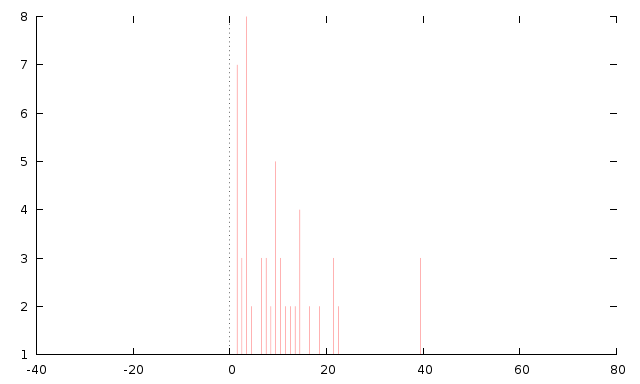
\includegraphics[scale=0.6]{times2-0.png}
\end{figure} 

\begin{figure}[H]
\centering
\caption{$N=2$, $\texttt{tfdepth}=2$}
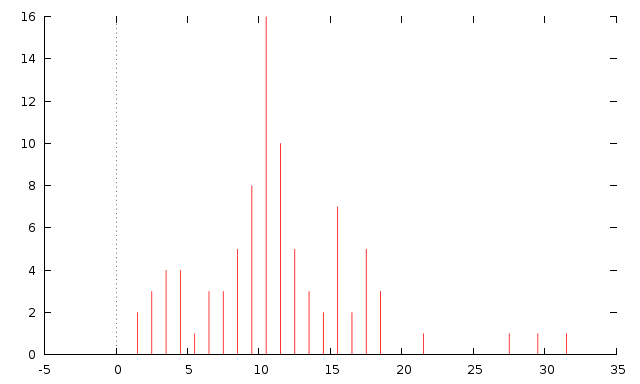
\includegraphics[scale=0.6]{times2-2.png}
\end{figure} 

\begin{figure}[H]
\centering
\caption{$N=2$, $\texttt{tfdepth}=4$}
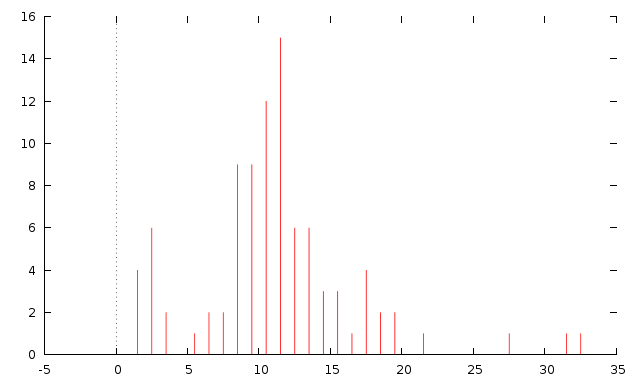
\includegraphics[scale=0.6]{times2-4.png}
\end{figure} 

\begin{figure}[H]
\centering
\caption{$N=2$, $\texttt{tfdepth}=8$}
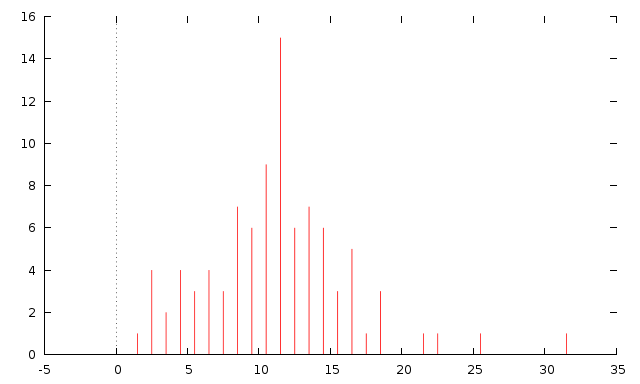
\includegraphics[scale=0.6]{times2-8.png}
\end{figure} 

\begin{figure}[H]
\centering
\caption{$N=2$, $\texttt{tfdepth}=16$}
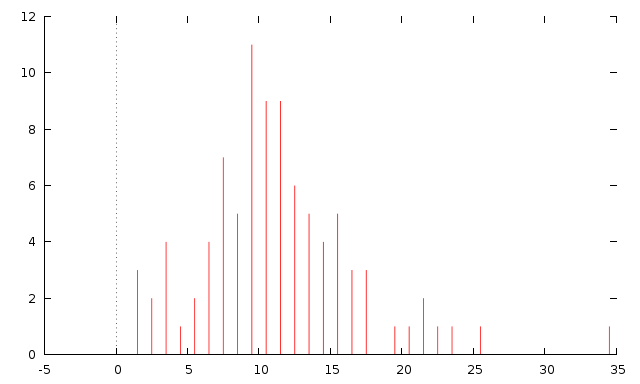
\includegraphics[scale=0.6]{times2-16.png}
\end{figure} 

\begin{figure}[H]
\centering
\caption{$N=4$, $\texttt{tfdepth}=0$}
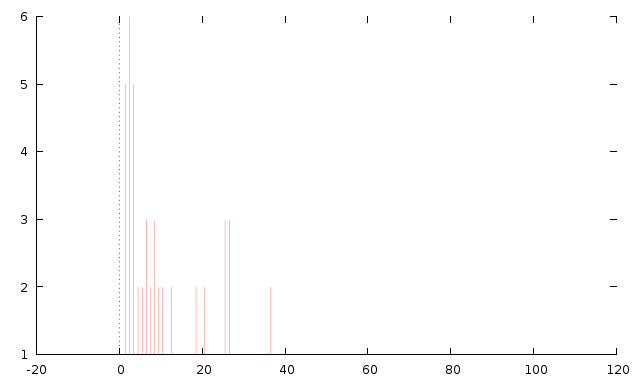
\includegraphics[scale=0.6]{times4-0.png}
\end{figure} 

\begin{figure}[H]
\centering
\caption{$N=4$, $\texttt{tfdepth}=2$}
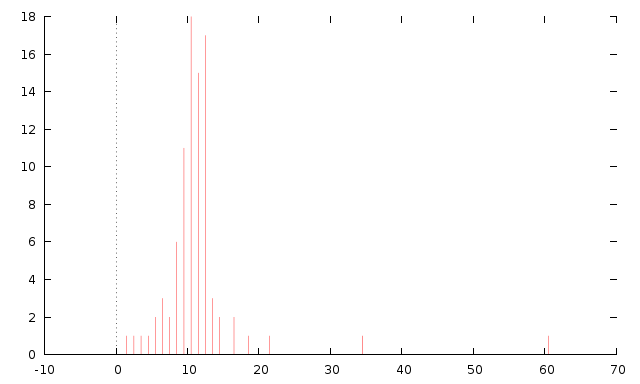
\includegraphics[scale=0.6]{times4-2.png}
\end{figure} 

\begin{figure}[H]
\centering
\caption{$N=4$, $\texttt{tfdepth}=4$}
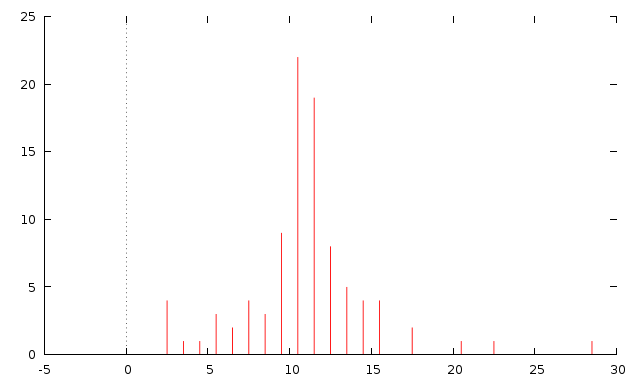
\includegraphics[scale=0.6]{times4-4.png}
\end{figure} 

\begin{figure}[H]
\centering
\caption{$N=4$, $\texttt{tfdepth}=8$}
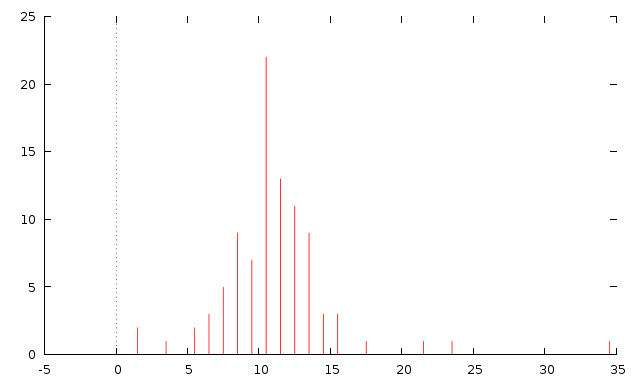
\includegraphics[scale=0.6]{times4-8.png}
\end{figure} 

\begin{figure}[H]
\centering
\caption{$N=4$, $\texttt{tfdepth}=16$}
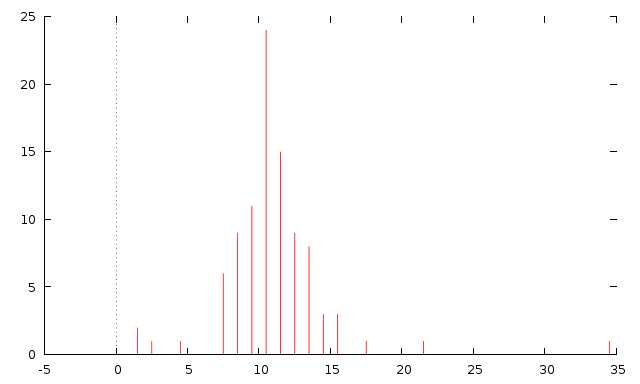
\includegraphics[scale=0.6]{times4-16.png}
\end{figure} 

\begin{figure}[H]
\centering
\caption{$N=8$,  $\texttt{tfdepth}=0$}
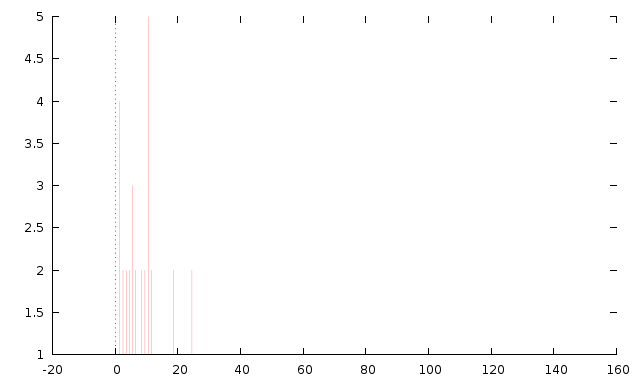
\includegraphics[scale=0.6]{times8-0.png}
\end{figure} 

\begin{figure}[H]
\centering
\caption{$N=8$, $\texttt{tfdepth}=0$, $T=10000$}
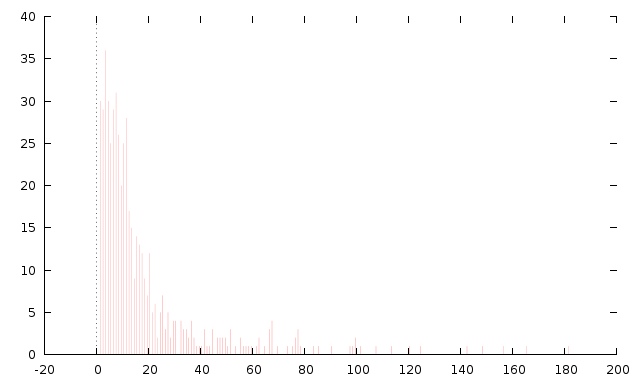
\includegraphics[scale=0.6]{times8-0-10000.png}
\end{figure} 


\begin{figure}[H]
\centering
\caption{$N=8$, $\texttt{tfdepth}=2$}
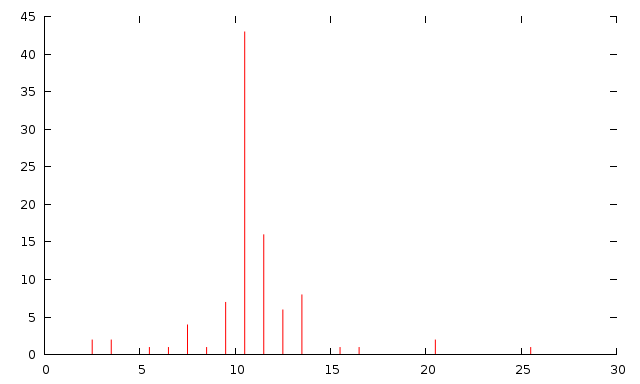
\includegraphics[scale=0.6]{times8-2.png}
\end{figure} 

\begin{figure}[H]
\centering
\caption{$N=8$, $\texttt{tfdepth}=4$}
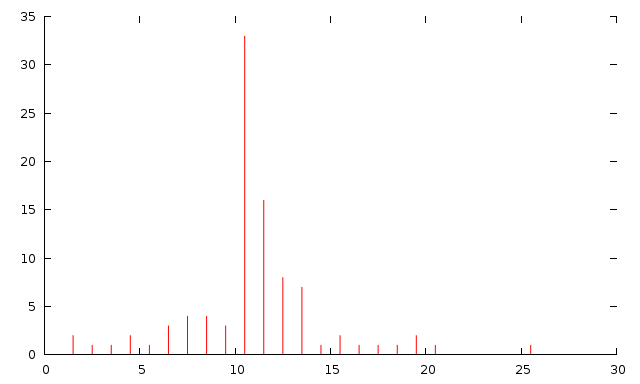
\includegraphics[scale=0.6]{times8-4.png}
\end{figure} 

\begin{figure}[H]
\centering
\caption{$N=8$, $\texttt{tfdepth}=8$}
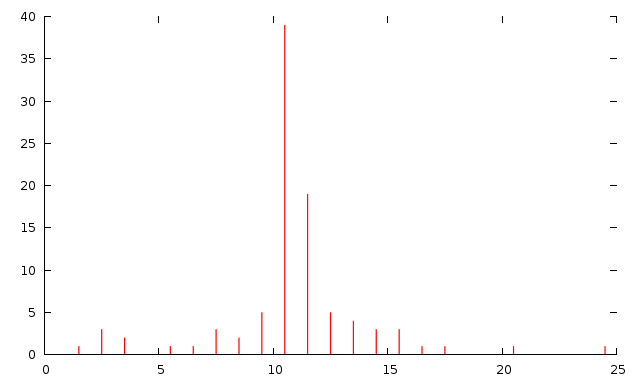
\includegraphics[scale=0.6]{times8-8.png}
\end{figure} 

\begin{figure}[H]
\centering
\caption{$N=8$, $\texttt{tfdepth}=16$}
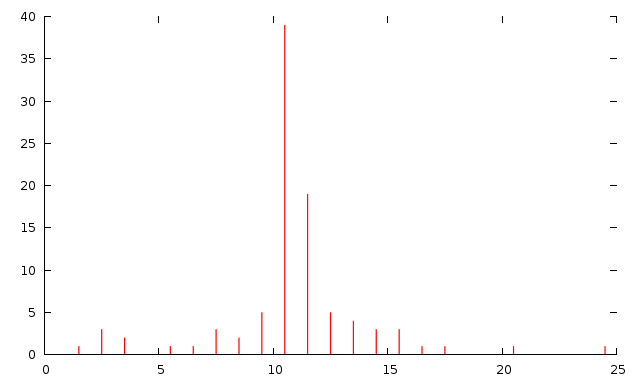
\includegraphics[scale=0.6]{times8-16.png}
\end{figure} 

\begin{figure}[H]
\centering
\caption{$N=8$, $\texttt{tfdepth}=16$, $T=2000$}
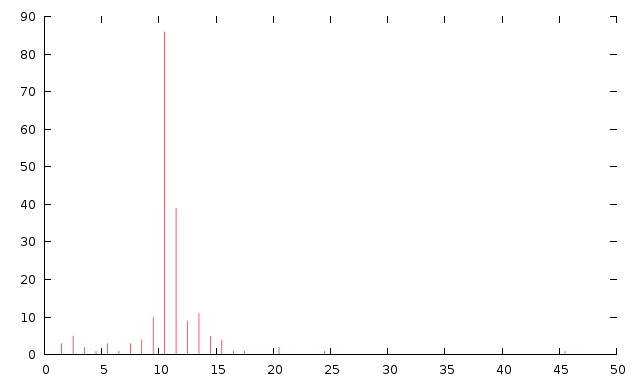
\includegraphics[scale=0.6]{times8-16-2000.png}
\end{figure} 

\begin{figure}[H]
\centering
\caption{$N=8$, $\texttt{tfdepth}=16$, $T=4000$}
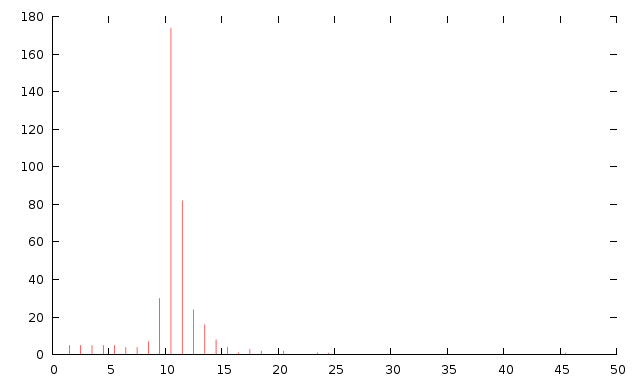
\includegraphics[scale=0.6]{times8-16-4000.png}
\end{figure} 

\begin{figure}[H]
\centering
\caption{$N=15$, $\texttt{tfdepth}=0$}
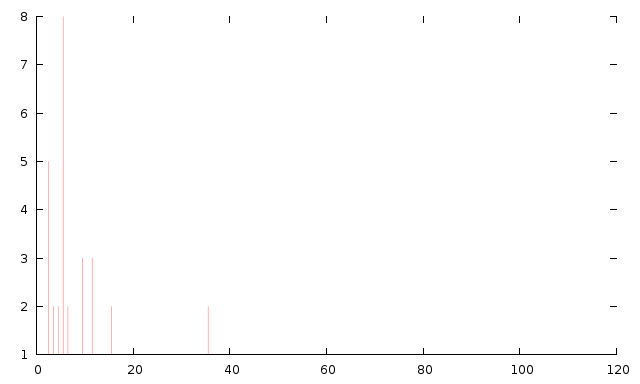
\includegraphics[scale=0.6]{times15-0.png}
\end{figure} 

\begin{figure}[H]
\centering
\caption{$N=15$, $\texttt{tfdepth}=2$}
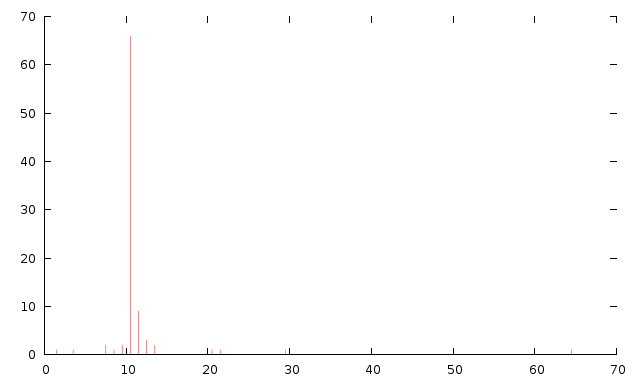
\includegraphics[scale=0.6]{times15-2.png}
\end{figure} 

\begin{figure}[H]
\centering
\caption{$N=15$, $\texttt{tfdepth}=4$}
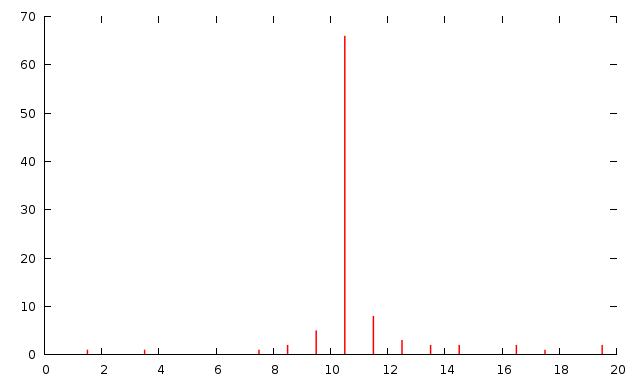
\includegraphics[scale=0.6]{times15-4.png}
\end{figure} 

\begin{figure}[H]
\centering
\caption{$N=15$, $\texttt{tfdepth}=8$}
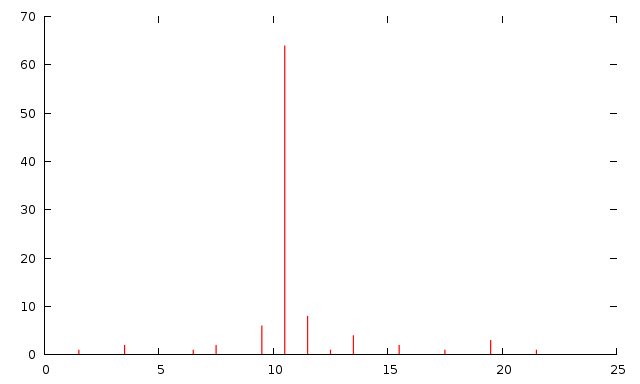
\includegraphics[scale=0.6]{times15-8.png}
\end{figure} 

\begin{figure}[H]
\centering
\caption{$N=15$, $\texttt{tfdepth}=16$}
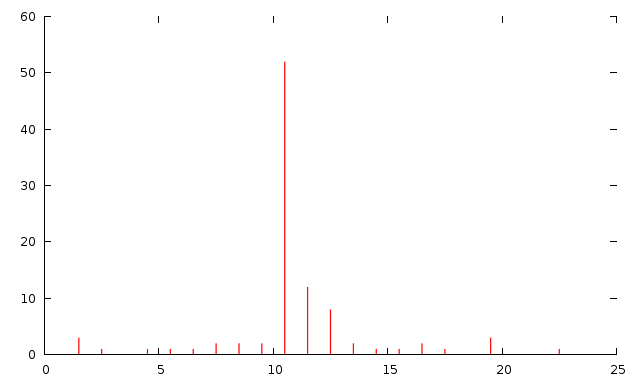
\includegraphics[scale=0.6]{times15-16.png}
\end{figure} 

\begin{table}[H]
\caption{Generated blocks number in dependence on $N$ and \texttt{tfdepth}}
\begin{center}
\begin{tabular}{|l|c|c|c|c|}
\hline
$\texttt{tfdepth}\backslash N$ & 2 & 4 & 8 & 15\\
\hline
single branch & 71 & 62 & 47 & 51 \\
1 & 89 & 92 & 96 & 97\\
2 & 91 & 90 & 97 & 92\\
4 & 94 & 95 & 96 & 97\\
8 & 94 & 95 & 96 & 97\\
16 & 92 & 96 & 96 & 97\\
\hline
\end{tabular}
\end{center}
\end{table}

We also simulate {\bf full} multibranch forging without specifying the \texttt{tfdepth} parameter for $2$ accounts. So the binary tree of blocks has been
built. This simulation is done to analyze whether the much better chain could be found if we don't restrict the number of blocks to forge to. The results
of simulation are below and are compared with the single branch forging (original) and with multibranch for different depths:

\begin{table}[H]
\caption{Number of the generated blocks in dependence on the time of simulation and \texttt{tfdepth} with $N=2$}
\begin{center}
\begin{tabular}{|l|c|c|c|c|}
\hline
$\texttt{tfdepth}\backslash T$ & 50 & 100 & 150 & 200\\
\hline
single branch & 2 & 5 & 7 & 13\\
1 & 4 & 7 & 14 & 18\\
10 & 4 & 8 & 14 & 18 \\
50 & 4 & 9 & 14 & 18 \\
100 & 4 & 9 & 14 & 18 \\
1000 & 4 & 9 & 15 & 18 \\
ignored ($=\infty$) & 4 & 9 & 15 & 19\\
\hline
\end{tabular}
\end{center}
\end{table}
 
The presented graphs demonstrate the following observable properties of multibranh forging:
\begin{itemize}
\item[1.] {The simulation confirms the results of the first article about single branch forging \url{http://www.scribd.com/doc/243341106/nxtforging-1}. 
The average block time goes to $2\tau$ when the number of uniform accounts goes to $\infty$.}
\item[2.] {The multibranch forging allows to have the average block time much closer to the specified $\tau$.}
\item[3.] {The distribution of block times becomes much more similar to gaussian with the multibranch.}
\item[4.] {The possibility of long tails decreases with the growing depth of tree forging. The max interval occurred doesn't exceed $5\tau$ in the most cases as 
for the single branch model it goes up to $18\tau$.}
\item[5.] {Longer runs save the shape of the distribution.}
\item[6.] {However the distribution dependence on the \texttt{tfdepth} parameter is not very high. The good results one can get just forging to the block with
maximum \texttt{baseTarget} from some set of the last blocks generated rather than to the last block in the longest chain.}
\item[7.] {The full multibranch forging takes a huge amount of computing power and has better but not amazing properties. So there is no need to use much power to do
the multibranch.}
\item[8.] {However it's obvious that an account which has more powerful computing node also has some benefits in comparison with other nodes because it could predict
more branches to somehow determine which branch will win in the longer run. That is the question for the future research 
still we don't like to transform the PoS systems to the PoW-like.}
\end{itemize}

\section{Conclusion and future work}
In this paper we demonstrated the ideas of multibranch forging and possible implementation approach using the proofs of code concept. 
Also the interpretation of the multibranch forging as a kind of TF is presented and definitely shows applicable results. The running simulating 
program is written basically in the Coq system and then extracted to the Haskell sources. All the simulation results are retrieved 
by the written program and plotted in the Gnuplot. The results of multibranch forging for different cases are presented with observable analysis. 
The future works include:
\begin{itemize}
\item[1.] {Research on the best algorithm for choosing the open blocks.}
\item[2.] {Research on the efficient algorithm for the tree rebalancing to present internal current vision for each account.}
\item[3.] {Research on the applicable fee distribution algorithm in the multibranch model.}
\item[4.] {The detailed description of the provable code approach and its usage to construct PoS systems to be issued as a separate paper.}
\item[5.] {Research and simulation of the system properties with additional features like transactions, changing connections etc.}
\item[6.] {Global research on the possible consensus in the multibranch systems as well as in more broad class of PoX systems.}
\end{itemize}     

\end{document}




